\section{Umsetzung}

\subsection{Allgemeines}
\frame{\frametitle{Tools \& System}
	\textbf{Tools}
	\begin{itemize}
		\item Code - Android Studio 1.5.1
		\item Dokumentation - TeXstudio 2.10.4
		\item UML Design - UMLet 14.2
		\item DB Design - DBDesigner 4
	\end{itemize}
	\textbf{Systemvoraussetzung (App)}
	\begin{itemize}
		\item Android Version 6.0 (API 23)
		\item Zugriff: Netzwerk
		\item Zugriff: Internet
		\item Zugriff: Externer Speicher
	\end{itemize}
}

\subsection{Code Design}
\frame{\frametitle{MVC Pattern}
	\begin{figure}
		\includegraphics[scale=1]{pic/MVC}
	\end{figure}
}

\frame{\frametitle{Model}
	\begin{figure}
		\includegraphics[scale=0.75]{pic/DBPattern}
	\end{figure}
}

\subsection{View}
\frame{\frametitle{View Steuerung}
	\begin{figure}
		\includegraphics[scale=0.5]{pic/Activities}
	\end{figure}
}

\frame{\frametitle{Startbildschirm}
	\begin{figure}
		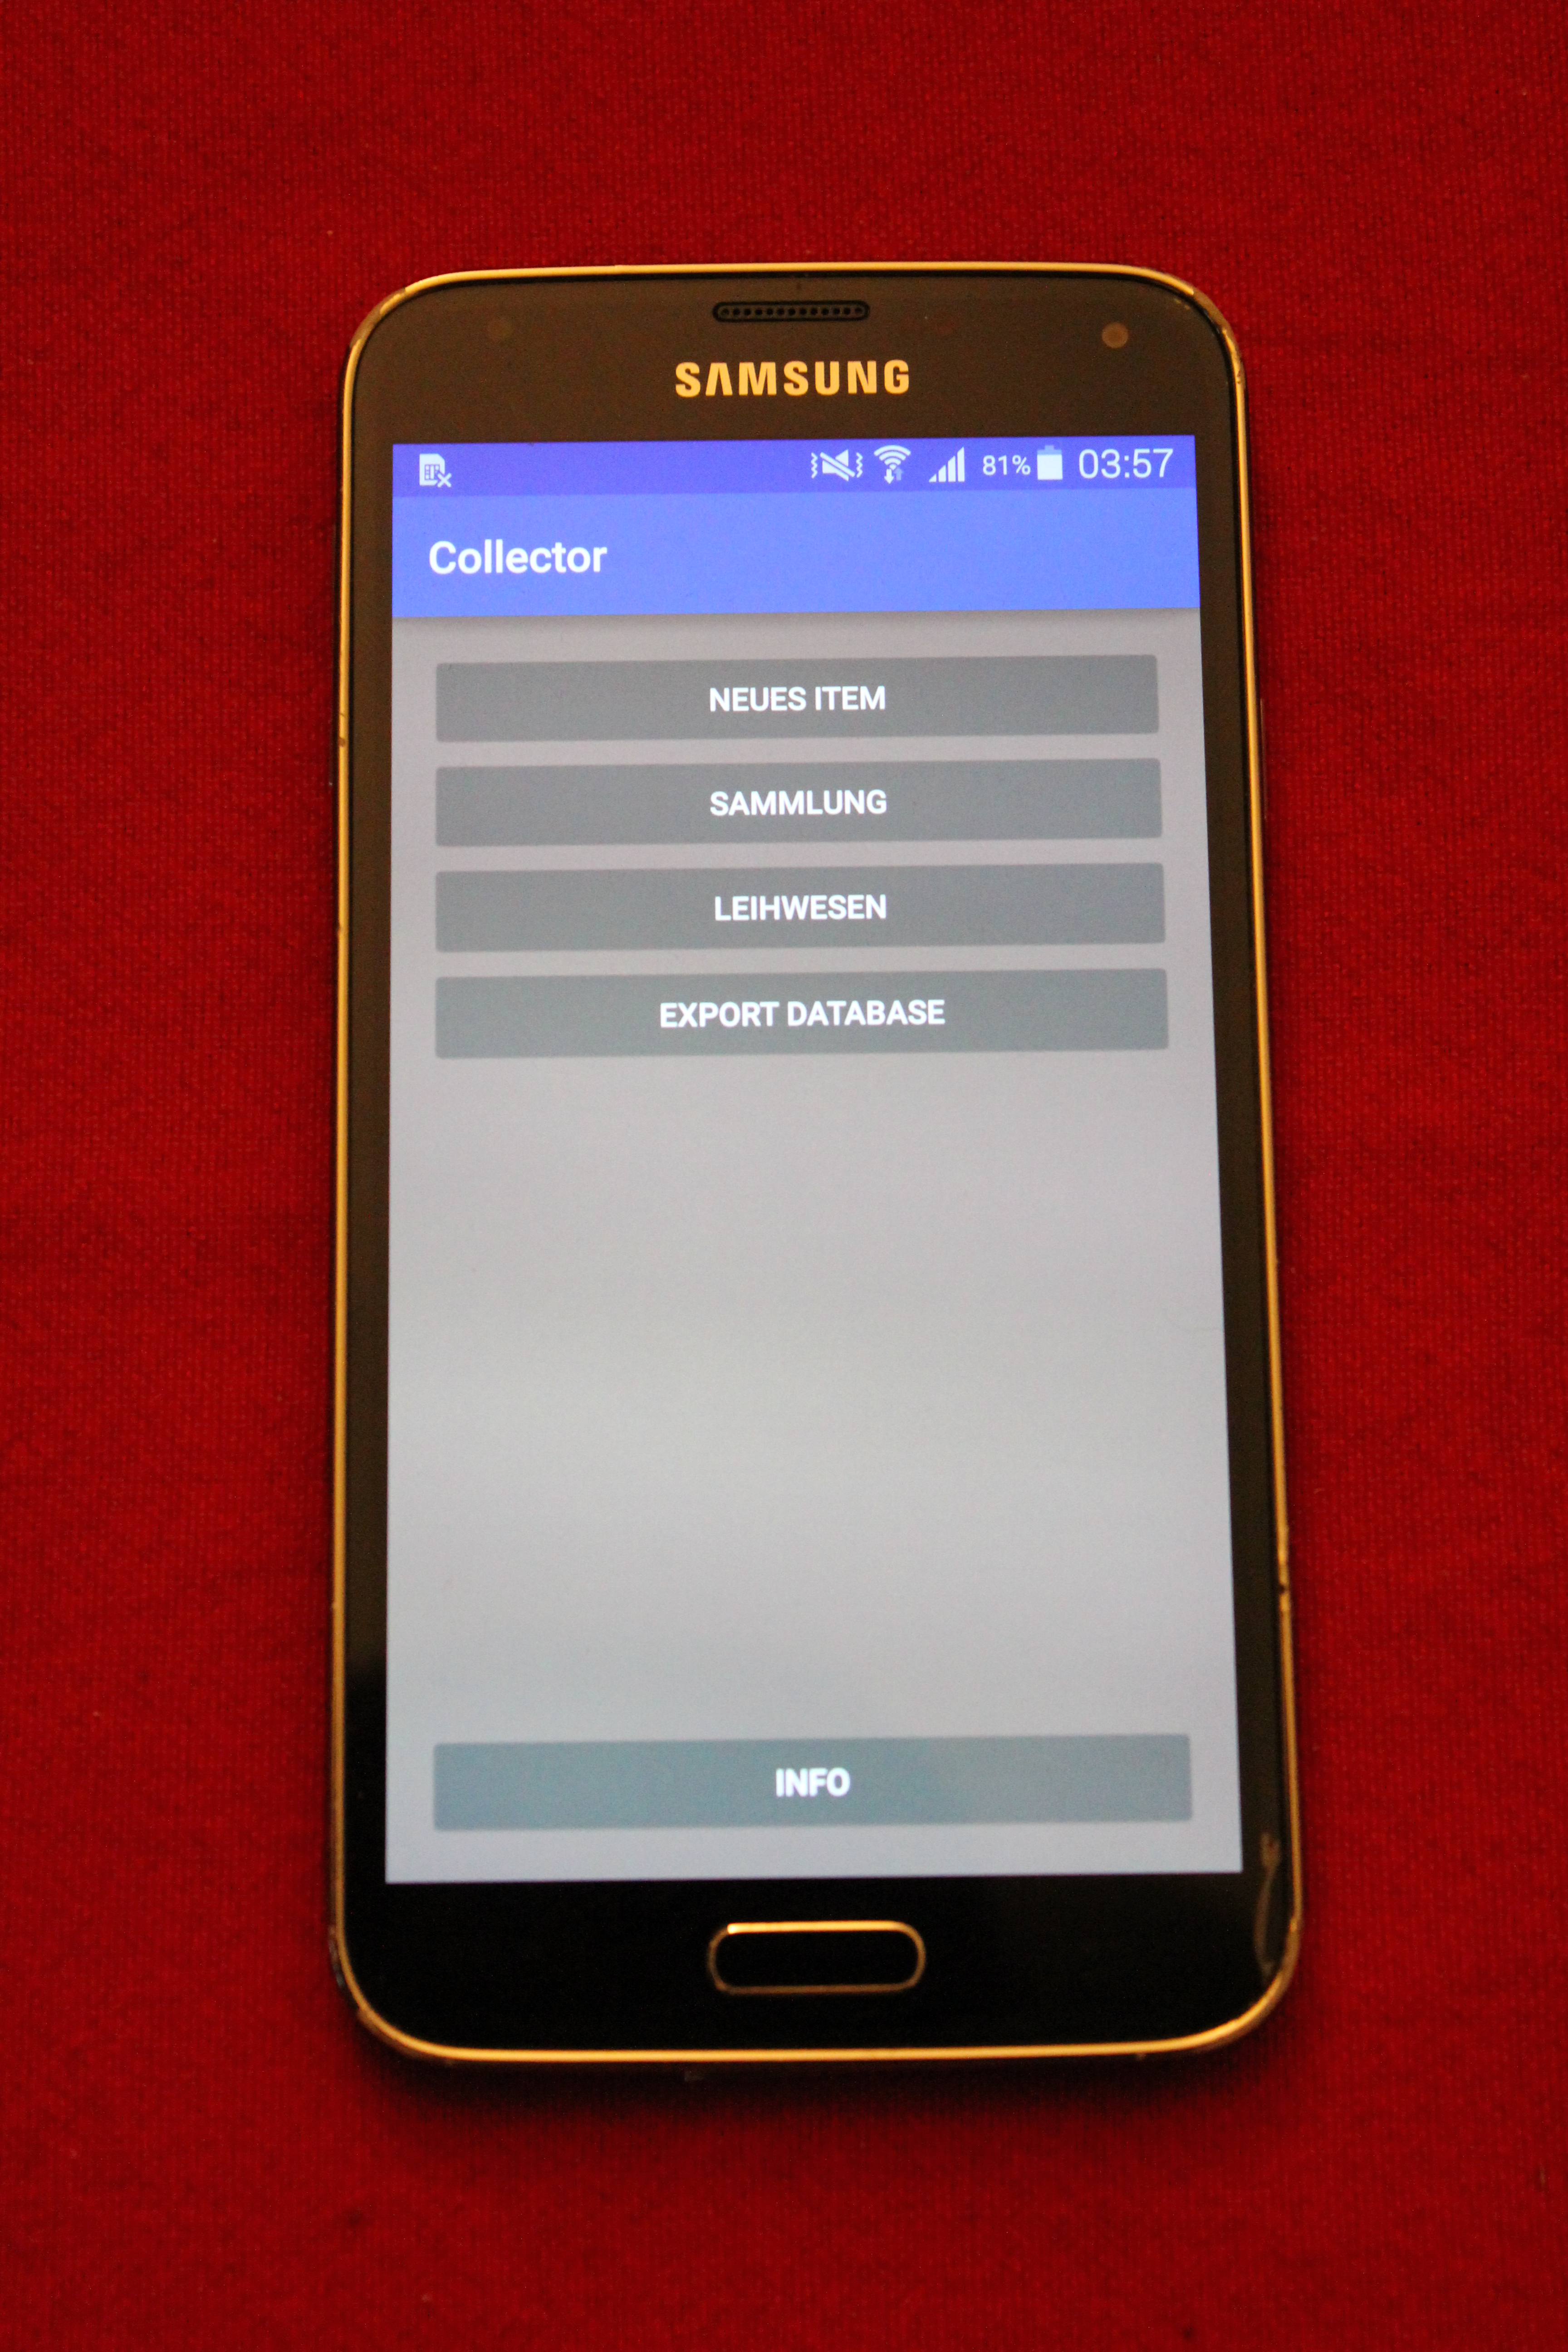
\includegraphics[scale=0.0375]{pic/HauptSCR}
	\end{figure}
}

\frame{\frametitle{Neues Item/Filter/Export}
	\begin{figure}
		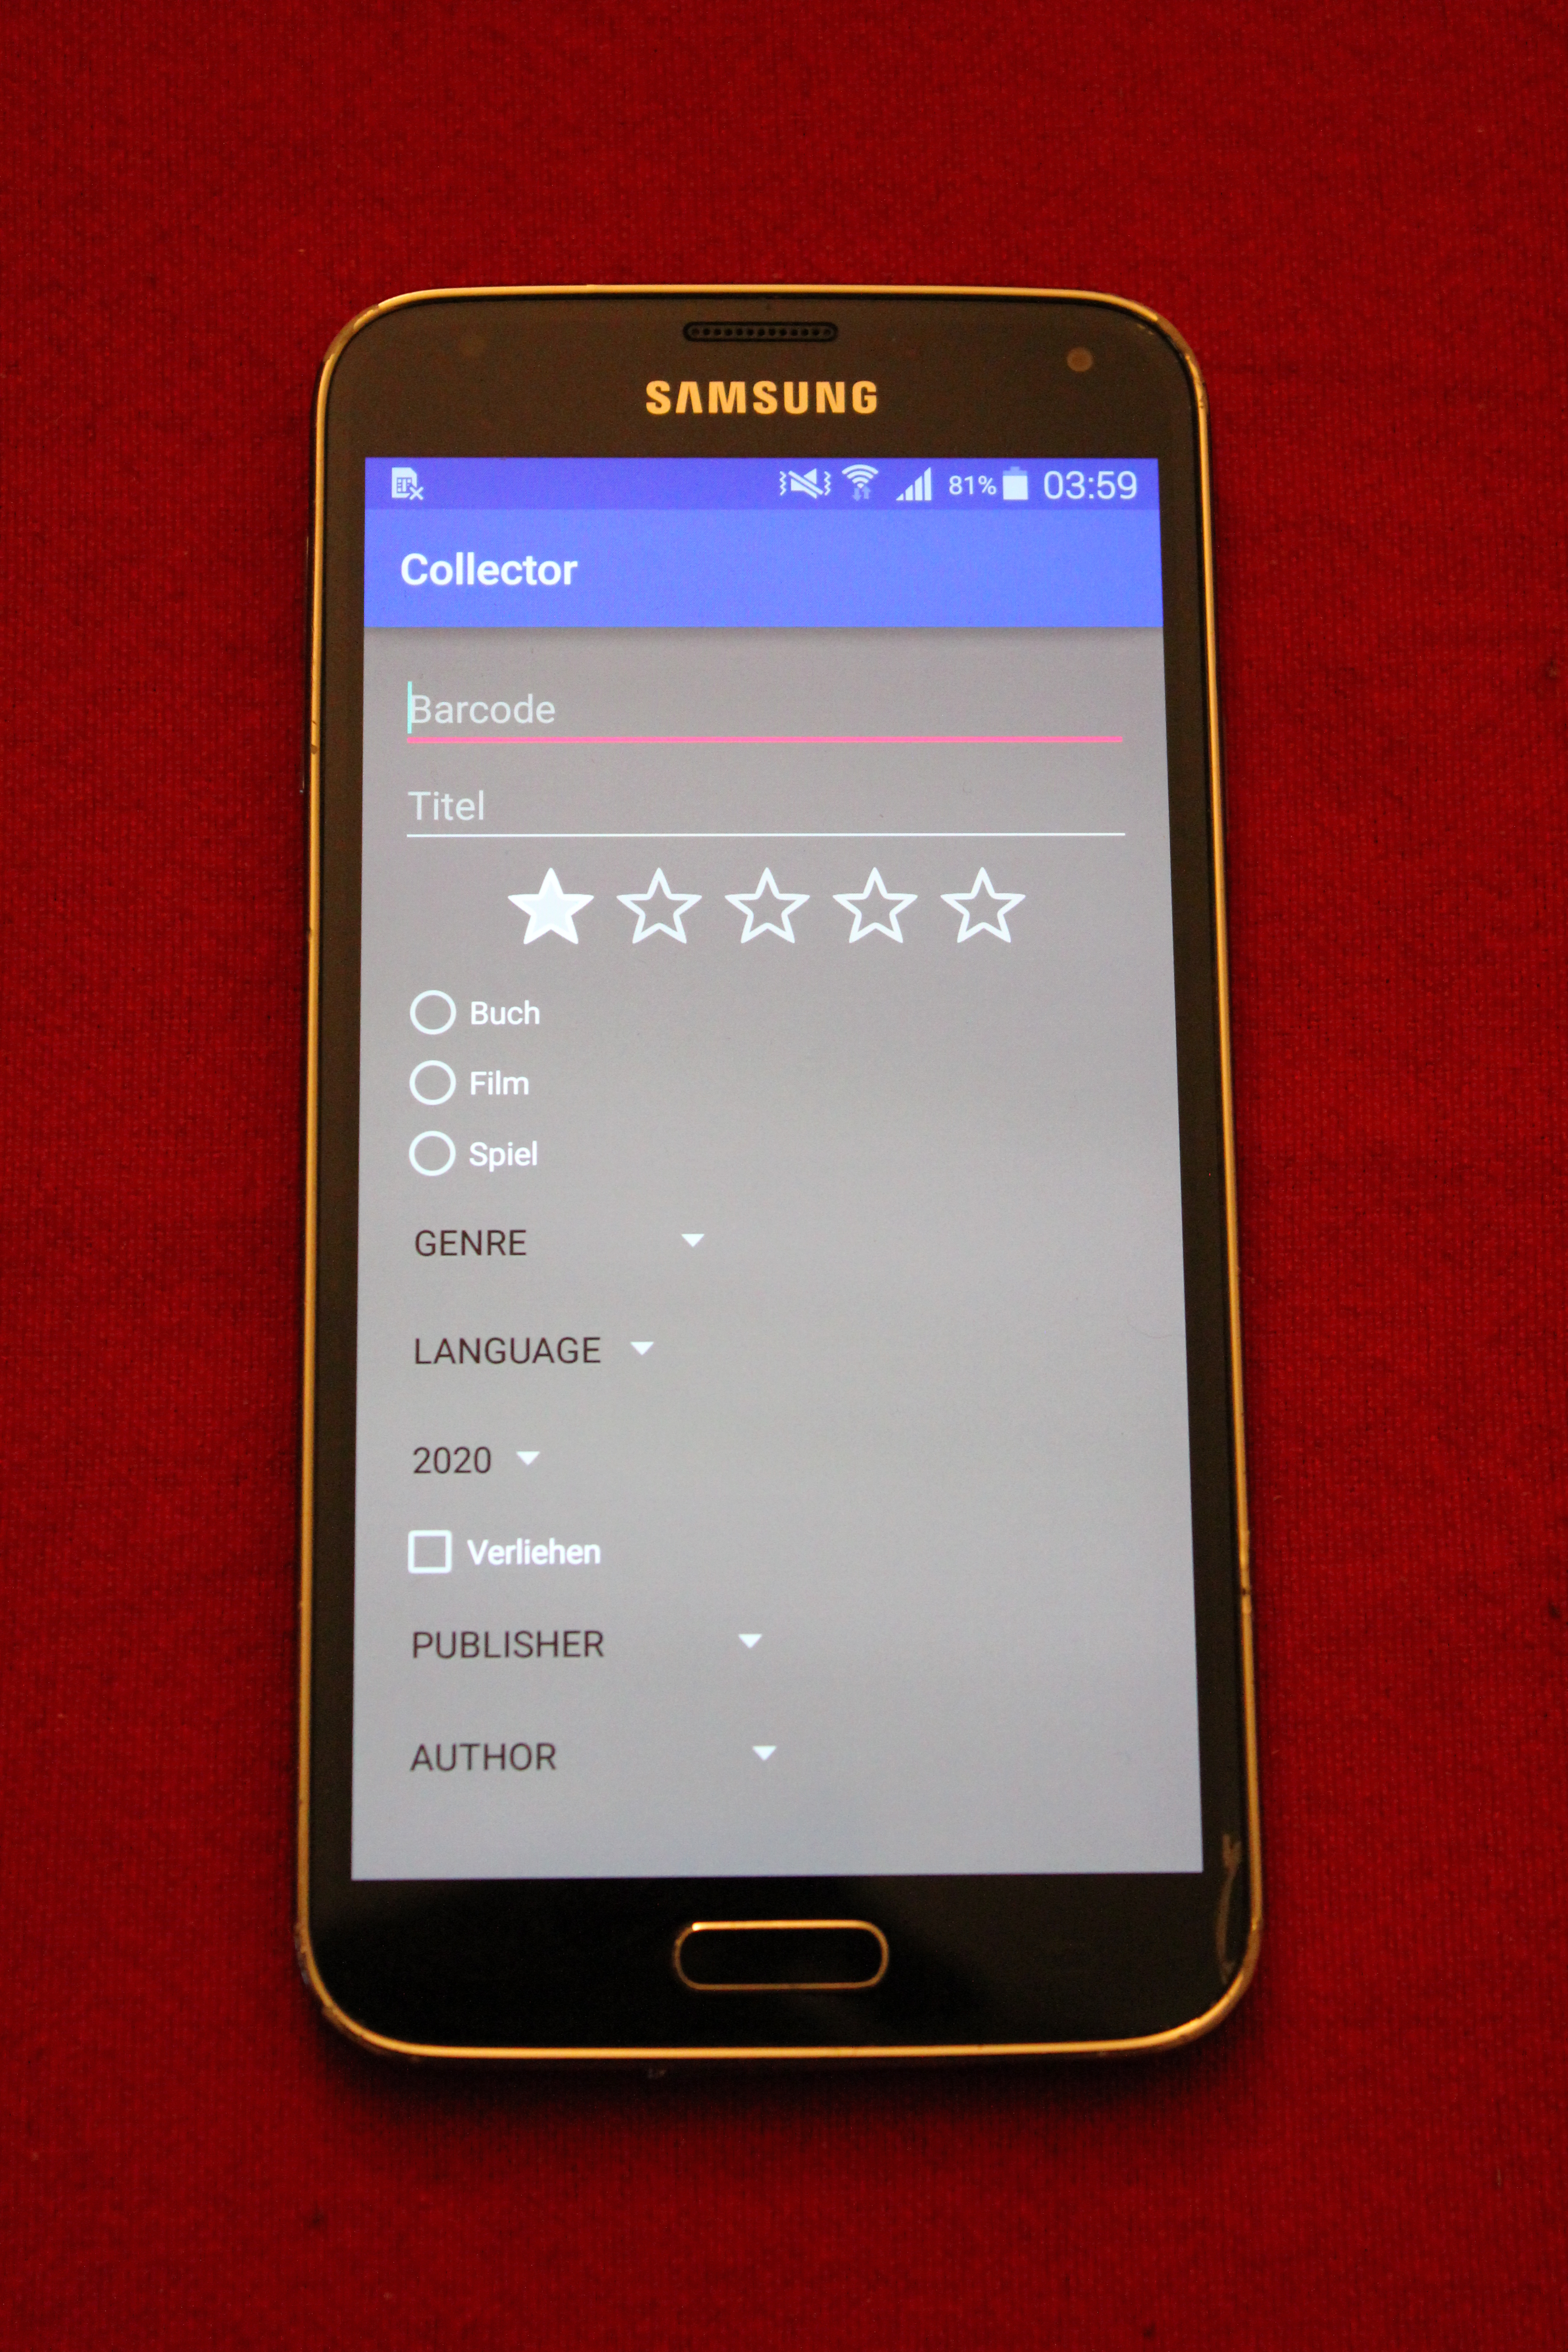
\includegraphics[scale=0.0375]{pic/New01SCR}
	\end{figure}
}

\frame{\frametitle{Neues Item/Filter/Export}
	\begin{figure}
		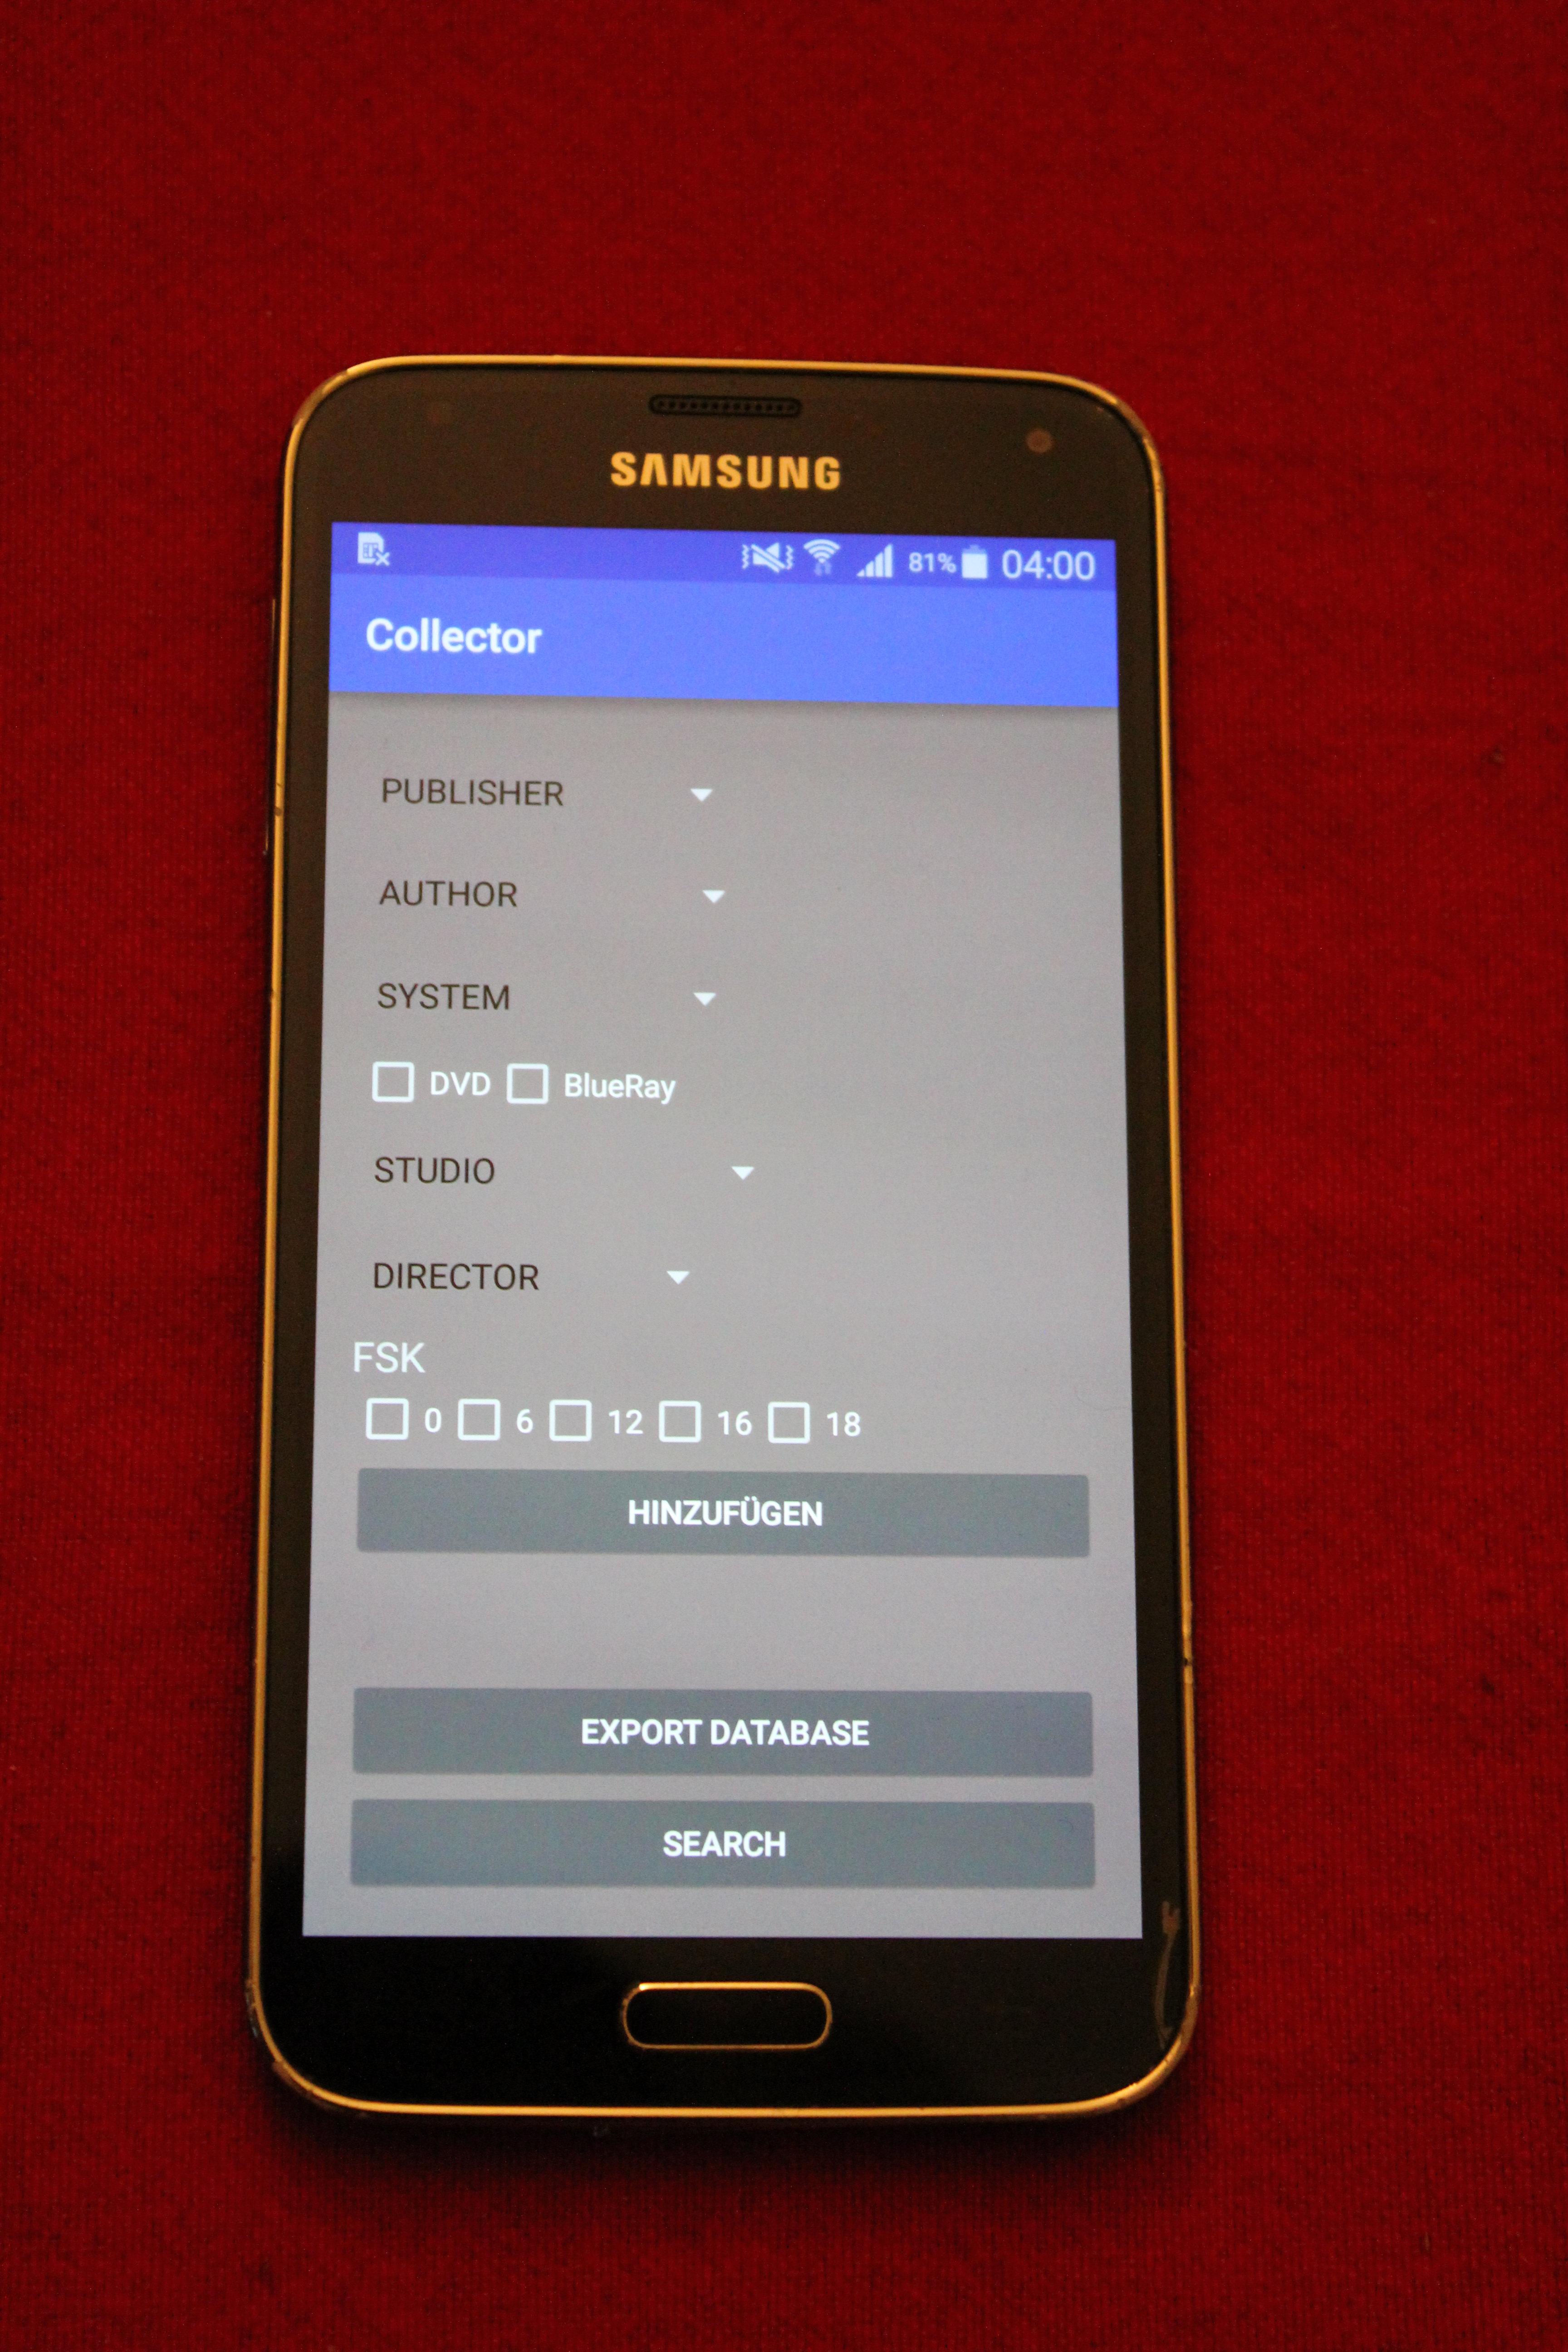
\includegraphics[scale=0.0375]{pic/New02SCR}
	\end{figure}
}

\frame{\frametitle{Button}
	\lstinputlisting[basicstyle=\tiny,frame=single,language=java,label=listener,caption=View: Button]{code/button.xml}
}

\frame{\frametitle{Button Listener}
	\lstinputlisting[basicstyle=\tiny,frame=single,language=java,label=listener,caption=Controller: Button Listener]{code/listenerDB.java}
}

\frame{\frametitle{Controller: ListView}
	\lstinputlisting[basicstyle=\tiny,frame=single,language=java,label=listener,caption=Controller: ListView]{code/ListView.java}
}